\documentclass[journal]{IEEEtran}
\usepackage[T1]{fontenc}
\usepackage{mathptmx}
\usepackage{amsmath,amssymb,amsthm}
\usepackage{graphicx,booktabs,multirow,array}
\usepackage{algorithm,algpseudocode}
\usepackage{cite,xcolor,microtype}
\usepackage{xr-hyper}
\usepackage[hidelinks]{hyperref}
\usepackage{stfloats,placeins,flushend}
\newcommand{\method}{\textsc{MAGIC}}
\newcommand{\E}{\mathbb{E}}
\newcommand{\PP}{\mathbb{P}}
\newcommand{\ind}{\mathbf{1}}
\newcommand{\pos}[1]{[#1]_+}
\newcommand{\Dataset}[1]{\texttt{\detokenize{#1}}}
\newtheorem{proposition}{Proposition}
\newtheorem{theorem}{Theorem}
\newtheorem{corollary}{Corollary}
\DeclareMathOperator*{\argmax}{arg\,max}
\graphicspath{{figures/}}
\setlength{\textfloatsep}{10pt plus 2pt minus 2pt}
\setlength{\floatsep}{8pt plus 2pt minus 2pt}
\setlength{\intextsep}{8pt plus 2pt minus 2pt}
\setlength{\emergencystretch}{1em}
\hyphenation{crowd-sourcing cali-bra-tion like-li-hood}
\renewcommand{\topfraction}{.95}
\renewcommand{\dbltopfraction}{.95}
\renewcommand{\textfraction}{.05}
\setcounter{topnumber}{3}
\setcounter{dbltopnumber}{3}
\makeatletter
\setlength{\@fptop}{0pt}
\setlength{\@fpsep}{14pt}
\setlength{\@dblfptop}{0pt}
\setlength{\@dblfpsep}{14pt}
\makeatother
\newcommand{\smalltable}{\footnotesize\setlength{\tabcolsep}{3.5pt}}

\makeatletter
\newcommand*{\addFileDependency}[1]{%
  \typeout{(#1)}\@addtofilelist{#1}%
  \IfFileExists{#1}{}{\typeout{No file #1.}}}
\makeatother
\newcommand*{\myexternaldocument}[2][]{%
  \externaldocument[#1]{#2}%
  \addFileDependency{#2.tex}%
  \addFileDependency{#2.aux}}
\myexternaldocument[supp-]{supplementary}
\begin{document}
\title{MAGIC: Adaptive Joint Calibration for Utility-Guided Gold Verification in Crowdsourcing}
\author{ Zhaori Guo, Qihao Song, Xia Du,~\IEEEmembership{Member,~IEEE}, Zhongqi Cai, Zheng Lin,~\IEEEmembership{Member,~IEEE}, Zihan Fang, \\Wei Ni,~\IEEEmembership{Fellow,~IEEE}, Jun Luo,~\IEEEmembership{Fellow,~IEEE}, Symeon Chatzinotas,~\IEEEmembership{Fellow,~IEEE} 


\thanks{Zhaori Guo, Qihao Song, Zhongqi Cai and Xia Du are with Xiamen University of Technology, Xiamen, China (e-mail: zhaoriguo@xmut.edu.cn; qihaosong@stu.xmut.edu.cn; zhongqicai@xmut.edu.cn; duxia@xmut.edu.cn).}%
\thanks{Z. Lin and S. Chatzinotas are with the Interdisciplinary Centre for Security, Reliability and Trust (SnT), University of Luxembourg, L-1855 Luxembourg, Luxembourg (e-mail: zhenglin@ieee.org; symeon.chatzinotas@uni.lu).}
\thanks{Z. Fang is with the Department of Computer Science, City University of Hong Kong, Kowloon, Hong Kong SAR, China (e-mail: zihanfang3-c@my.cityu.edu.hk).}
\thanks{Wei Ni is with the School of Engineering, Edith Cowan University, Perth, WA 6027, Australia (email: wei.ni@ieee.org).}
\thanks{Jun Luo is with the College of Computing
and Data Science, Nanyang Technological University, Singapore (e-mail: junluo@ntu.edu.sg).}
\thanks{(Corresponding author: Zhongqi Cai and Zheng Lin)}%
}
\maketitle
\begin{abstract}
A requester with crowdsourced predictions can deliver a label, reject it, or pay for verification. When verification costs more than the reward on its own task, its value depends on which other delivery decisions the observed label changes. MAGIC (Model Averaging for Gold Investment and Calibration) estimates this value by averaging over calibration hypotheses and over partitions of a task pool into contexts. Each purchase updates both the reliability of the fixed predictions and the extent to which tasks share calibration. Posterior utility cross moments give an exact one-step score for acquisition and stopping. We bound the value transferred to each task by its posterior dependence and its distance from the delivery threshold. The bound is exact for binary query outcomes. Across 15 real datasets and 13 aggregation baselines, mean net utility increases from 1.3527 to 1.9294 per task (42.63\%) over calibrated selective delivery without additional verification. Changes to unverified deliveries account for 82.94\% of the gross gain.
\end{abstract}
\begin{IEEEkeywords}
Crowdsourcing, truth inference, Bayesian model averaging, value of information, selective prediction, gold-label verification.
\end{IEEEkeywords}

\section{Introduction}
\IEEEPARstart{C}{rowdsourcing} aggregates noisy annotations from imperfect contributors into task predictions that support data labeling, information integration, and decision making~\cite{zheng2017truth}. Even strong aggregators leave some predictions wrong, and the loss from delivering an incorrect label can far exceed the reward for a correct one. A requester holding a pool of aggregated predictions therefore faces an economic decision: each prediction can be delivered as it is, withheld, or verified by purchasing a trusted gold label, whose price can exceed the reward of the task it resolves. Under a limited budget, the requester must decide which predictions to verify and which of the others to deliver by weighing reliability, task-specific consequences, and verification costs.

\begin{figure*}[!t]
\centering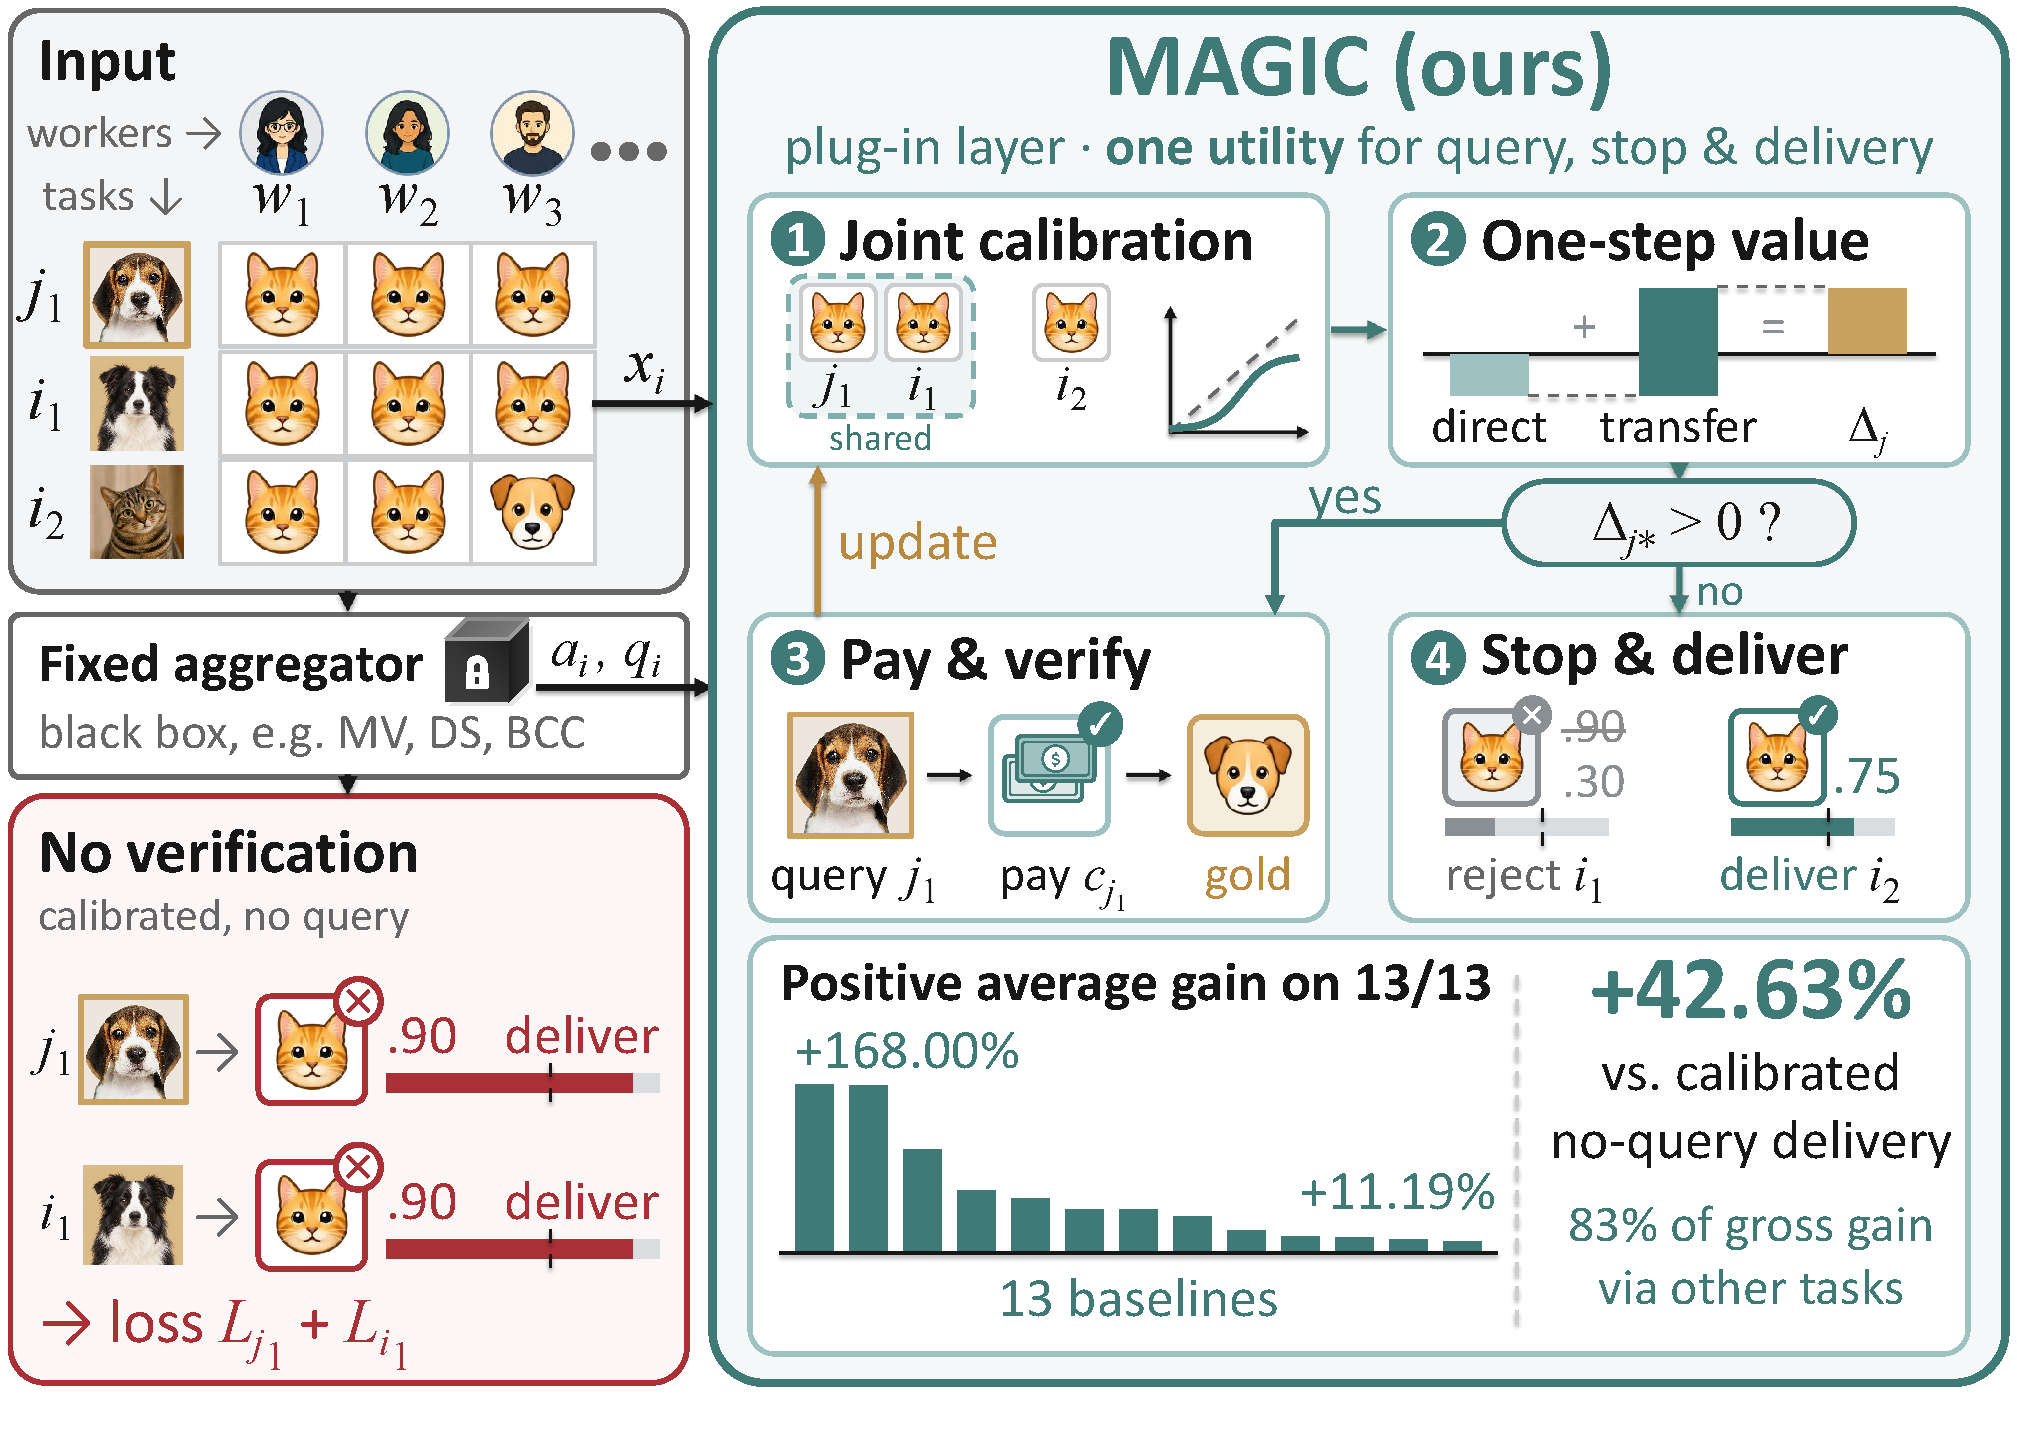
\includegraphics[width=.87\textwidth]{intro.pdf}
\caption{Motivating example. Delivering the confident aggregator labels of $j_1$ and $i_1$ without verification incurs two losses. MAGIC verifies $j_1$; the gold label updates calibration and sharing, so MAGIC rejects $i_1$ and delivers $i_2$. Bottom: average gains over the 13 baselines.}
\label{fig:intro}
\end{figure*}

Consider the two high-confidence predictions in Fig.~\ref{fig:intro}. Buying the label of $j_1$ resolves one error. If the same source of overconfidence affects $i_1$, that observation also prevents a second costly delivery. Two models can assign the same confidence to both predictions yet disagree about the value of buying $j_1$: under independent calibration, its label tells the requester nothing about $i_1$. Even under shared calibration, a change in confidence has economic value only when it changes the delivery decision.

MAGIC models both sources of uncertainty. A finite bank describes how confidence maps to correctness, and a tree over observable task features describes which tasks might share that mapping. Each purchased label updates the weights of both the calibration hypotheses and the sharing structures. This construction adds verification and selective delivery to any aggregator that supplies fixed predictions and class probabilities.

Our contributions are threefold.
\begin{itemize}
\item We formulate verification, stopping, and delivery under one budgeted utility objective. The joint calibration model gives exact one-step query values from posterior cross moments.
\item We characterize how a tree split changes information transfer even when initial marginal predictions agree. A margin-dependent bound isolates the posterior changes that can reverse a delivery decision and is attained for binary observations.
\item Across 15 datasets and 13 aggregators, every aggregator gains on average. Experiments on acquisition rules, verification prices, noisy gold labels, and pool size identify when the gain comes from correcting purchased labels and when it comes from revising other deliveries.
\end{itemize}


\section{Related Work}
\label{sec:related}

\subsection{Truth Inference and Calibration}
Truth inference models the reliability of workers and the difficulty of their tasks~\cite{dawid1979maximum,whitehill2009whose}. Mixture models extend inference to multilabel data~\cite{zhang2021multilabel}, while object--source graphs, bipartite attention, and graph contrastive learning capture relationships among workers, sources, and tasks~\cite{wu2023tira,liu2025bat,liu2024govern}. Other formulations accommodate domain constraints, changing source dependencies, and joint maximum likelihood estimation~\cite{ye2022constrained,zhang2026reliable,xiao2023joint}. Generative aggregation handles sentence-level answers~\cite{wang2023generative}.

Uncertainty estimates also depend on how models handle noise. Sparse worker weighting and loss thresholding downweight unreliable observations~\cite{yu2023robust,yang2024dynamic}. Transition models account for annotator-dependent noise and mixed noise types~\cite{li2024transferring,xia2023extended}. Variational models estimate predictive uncertainty, and nonparametric Bayesian models infer item-level features~\cite{morales2022scalable,stinson2025nonparametric}, and label propagation and pretrained aggregation pool evidence across sparse annotation matrices or task pools~\cite{zhang2025eldp,liu2026crowdfm}. MAGIC takes the resulting labels as fixed. It combines probability calibration~\cite{guo2017calibration} and selective prediction~\cite{geifman2017selective} with recursive pooling and splitting, a construction related to Bayesian context trees~\cite{kontoyiannis2022bayesian}.

\subsection{Budget-Constrained Label Acquisition}
Active multilabel consensus chooses sample--label--worker combinations~\cite{yu2021active}. Quality-aware assignment, crowd-based data cleaning, and cross-domain worker selection account for differences in worker accuracy and experience~\cite{gao2021quality,zhang2022cleaning,sun2024cross}. In sequential settings, the optimistic knowledge gradient ranks tasks by the possible improvement from another annotation~\cite{chen2013optimistic}, while multi-advisor policies trade the expected value of advice against its price and uncertainty about advisor reliability~\cite{guo2023maddm,guo2025cautious}. Hierarchical labeling similarly combines inexpensive predictions with selectively acquired stronger labels~\cite{zhang2025lmcrowd}.

The closest decision criteria value information through its effect on subsequent actions~\cite{kapoor2007selective} or distinguish the local and global effects of an expert label~\cite{liu2015boosting}. In our setting, verification earns a known reward on the purchased task and can change which fixed predictions are profitable to deliver elsewhere in the pool. Section~\ref{sec:experiments} compares these acquisition principles using the same task pools and budgets.


% ===== PROBLEM =====
\section{Problem Formulation}
\label{sec:problem}
\paragraph{Tasks, actions, and utilities}
We consider $n$ tasks with unknown reference labels $Y_i\in\{1,\ldots,C\}$. For each task $i$, the public inputs are an upstream probability vector $q_i$, a fixed predicted label $a_i$, annotation summaries $x_i$, a correct-delivery reward $r_i>0$, and a gold-verification price $c_i>0$. Let $L_i(a_i,y)\ge0$ be the loss for delivering $a_i$ when the truth is $y$, with $L_i(a_i,a_i)=0$. The utility of an unverified delivery is
\begin{equation}
 U_i(y)=r_i\ind\{y=a_i\}-L_i(a_i,y).
 \label{eq:utility}
\end{equation}
Rejecting a task yields zero. Purchasing a perfect gold label reveals $Y_i$ and permits delivery of the verified answer, which earns $r_i$ and costs $c_i$. The label of an unqueried task remains fixed: the decision layer chooses between delivery and rejection, not among alternative class labels.

\paragraph{Realized return}
For a purchased set $Q$ and an unqueried delivery set $S\subseteq[n]\setminus Q$, the realized return is
\begin{equation}
 R(Q,S,Y)=\sum_{i\in Q}(r_i-c_i)+\sum_{i\in S}U_i(Y_i),
 \label{eq:return}
\end{equation}
subject to the budget constraint $\sum_{i\in Q}c_i\le B$. Costs are charged for actual purchases, not for unused budget, and the reported net utility divides this return by the full pool size $n$. All candidate identities and features are public, but reference labels enter acquisition only through paid queries.

\paragraph{Prepaid training labels}
Some upstream models require paid training labels. Let $Q_{\rm tr}$ be their fixed training set and $C_{\rm tr}=\sum_{i\in Q_{\rm tr}}c_i$. These tasks are already verified, contribute the same return and consume the same budget on both sides of a paired comparison, and are removed from the candidates. The post-training decision problem thus operates on $[n]\setminus Q_{\rm tr}$ with budget $B-C_{\rm tr}$, while normalization still uses the original $n$; MAGIC does not reuse these labels as calibration observations. This bookkeeping is essential for the paid-training LAGNN adaptation.

\paragraph{Terminal delivery}
Let $H$ denote the paid calibration history, $R_H$ the remaining tasks, and $\mu_i(H)=\E[U_i(Y_i)\mid H]$. Delivery decisions are separable across tasks, so the optimal immediate delivery under a specified predictive model and its value are
\begin{equation}
 S(H)=\{i\in R_H:\mu_i(H)>0\},\qquad
 T(H)=\sum_{i\in R_H}\pos{\mu_i(H)}.
 \label{eq:terminal}
\end{equation}
Zero-utility ties are rejected by the implementation. With a constant incorrect-label loss $\ell_i$, the rule reduces to the threshold $P(Y_i=a_i\mid H)>\ell_i/(r_i+\ell_i)$; heterogeneous losses require the full class distribution in~\eqref{eq:utility}. The main notation is summarized in Supplementary Table~\ref{supp-tab:notation}.

\paragraph{Reference policy}
The experimental no-additional-query reference delivers $S(\varnothing)$ under the default MAGIC prior and retains any paid training tasks. The primary increment thus measures additional verification and the delivery changes it induces, relative to a reference that is already selective and prior-calibrated. When an ablation changes the prior or the delivery rule, we also report its own no-query reference, but we compare methods through final utility or a common reference.

% ===== METHOD =====
\section{The MAGIC Framework}
\label{sec:framework}

Figure~\ref{fig:framework} follows one purchase from candidate scoring to final delivery. The bank specifies the possible calibration errors, the tree specifies how tasks share them, and paid labels update both.

\begin{figure*}[t]
\centering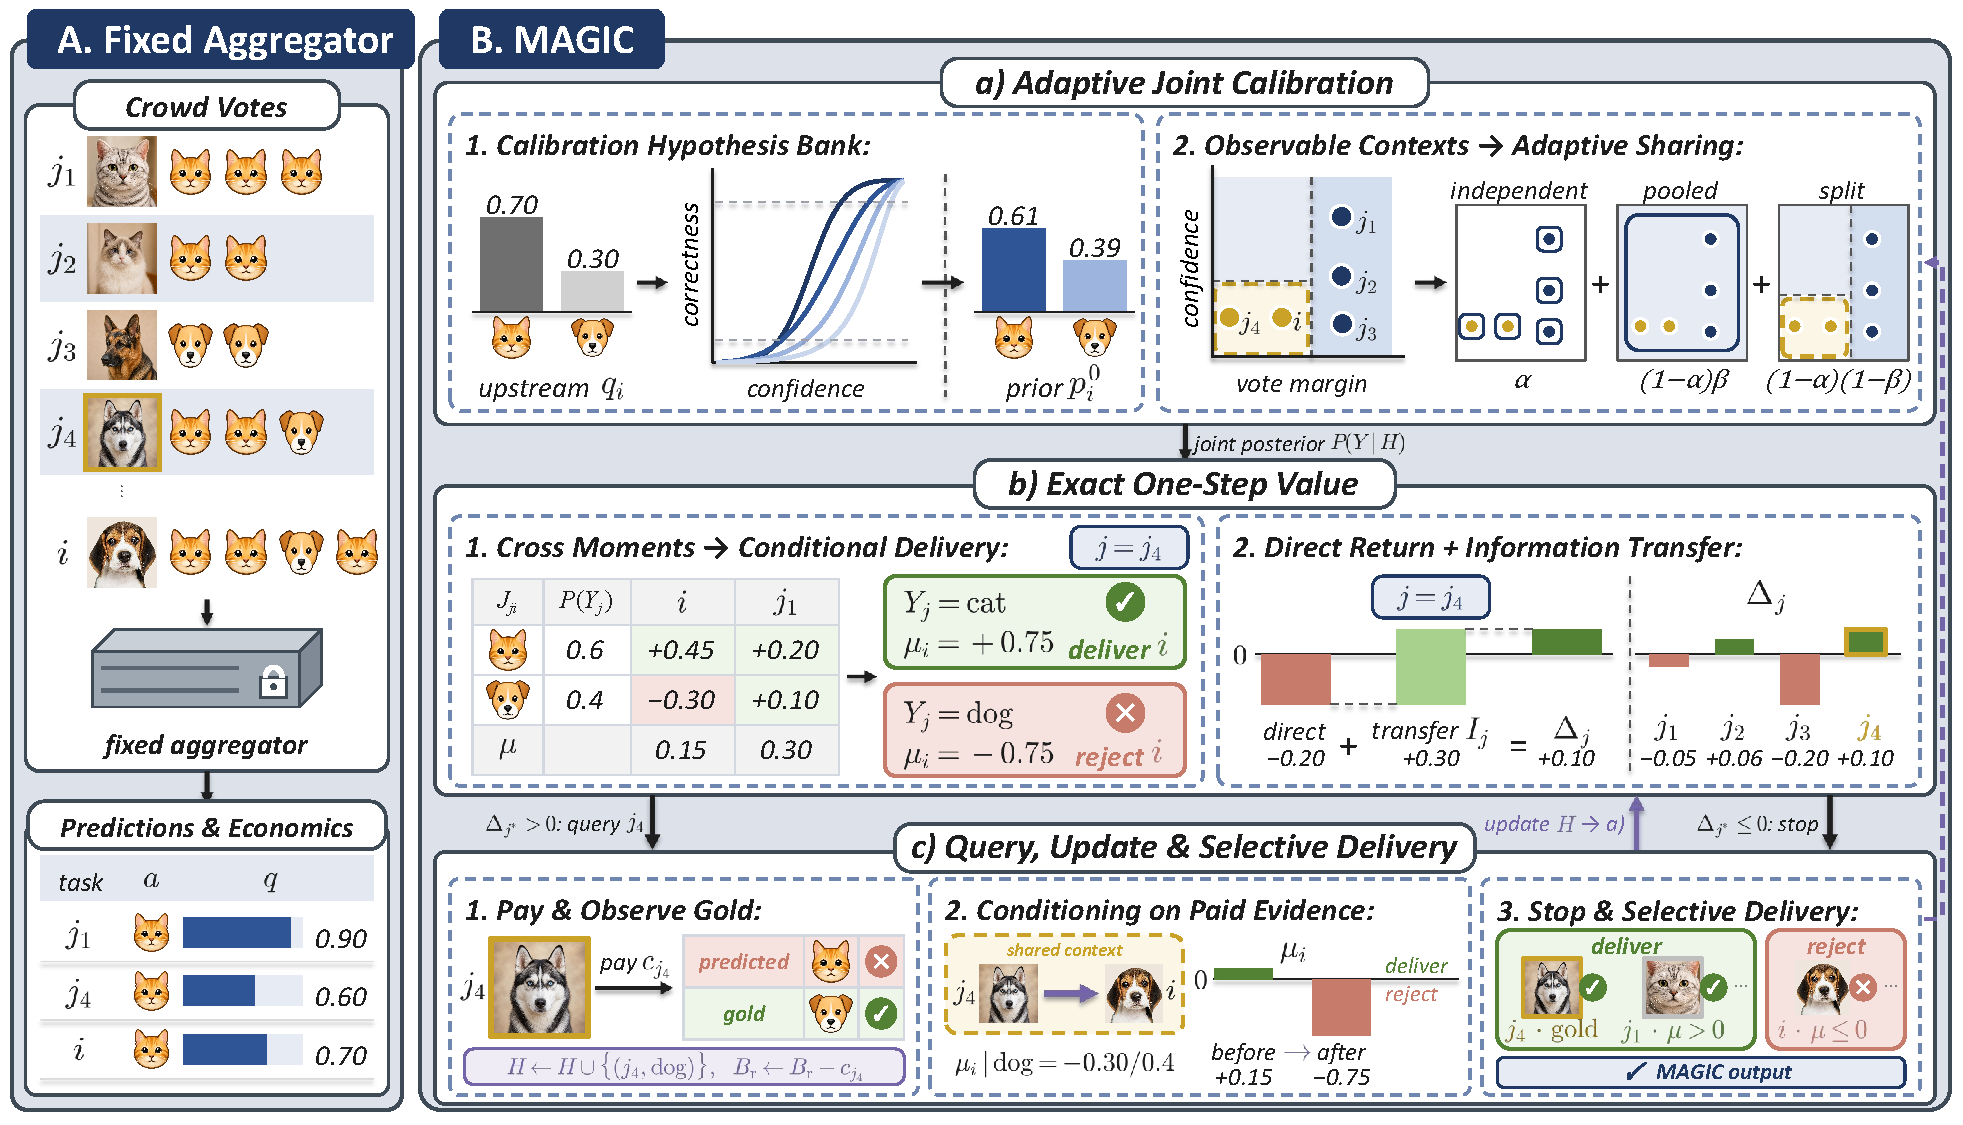
\includegraphics[width=\textwidth]{framework.pdf}
\caption{Overview of MAGIC. Only paid query outcomes update the joint posterior, and one terminal utility drives query values, stopping, and selective delivery. Sealed reference labels are used only for offline evaluation.}
\label{fig:framework}
\end{figure*}


\subsection{Finite Bank of Calibration Hypotheses}
\label{sec:bank}

Upstream probabilities may be miscalibrated in ways that are unknown before any gold label is purchased. We therefore treat the reliability of each fixed label as uncertain and describe the possible forms of miscalibration by a finite bank of calibration hypotheses, each of which specifies a class distribution $p_{hi}$ for every task $i$. Because a hypothesis applies to many tasks at once, a gold label that supports or contradicts it on one task also changes the predicted reliability of the others; Section~\ref{sec:context} specifies which tasks share hypotheses.

\paragraph{Two hypothesis families}
Let $s_i=q_i(a_i)$, clipped to $[\kappa,1-\kappa]$ with a small $\kappa>0$. The bank $\mathcal{H}=\mathcal{H}_{\mathrm{conf}}\cup\mathcal{H}_{\mathrm{const}}$ contains two families of hypotheses.

Each confidence-dependent hypothesis $h\in\mathcal{H}_{\mathrm{conf}}$ maps the upstream confidence to
\begin{equation}
    p_{hi}(a_i)
    =\sigma\bigl(t_h\operatorname{logit}(s_i)+b_h\bigr),
    \label{eq:calibrator}
\end{equation}
where $\sigma$ is the logistic function, and the slope $t_h$ and offset $b_h$ range over a finite grid $\mathcal{G}_t$ of positive values and a finite grid $\mathcal{G}_b$. The slope sharpens or flattens the confidence, the offset corrects systematic over- or underconfidence, and $(t_h,b_h)=(1,0)$ leaves the upstream confidence unchanged.

Some aggregators report nearly saturated confidence even for wrong predictions. The first family cannot lower the correctness probability much in that case: with the default grids, all its hypotheses exceed 0.94 at $s_i=1-\kappa$. Each confidence-independent hypothesis $h\in\mathcal{H}_{\mathrm{const}}$ therefore ignores $s_i$ and assigns
\begin{equation}
    p_{hi}(a_i)=\pi_h,\qquad
    \pi_h\in\mathcal{P},
    \label{eq:constant-calibrator}
\end{equation}
where $\mathcal{P}\subset(0,1)$ is a finite set of candidate correctness probabilities. We refer to this second family as the \emph{broad} hypotheses.

\paragraph{Residual distributions}
Both families must also spread the remaining mass over the incorrect classes. For $y\ne a_i$,
\begin{equation}
    p_{hi}(y)=\bigl(1-p_{hi}(a_i)\bigr)\,\nu_{hi}(y),
    \label{eq:residual}
\end{equation}
where $\nu_{hi}$ is either the upstream residual $q_i(y)/\sum_{y'\ne a_i}q_i(y')$, which keeps the aggregator's ranking of the other classes, or the uniform residual $1/(C-1)$. This choice matters when wrong-label losses differ across true classes.

\paragraph{Prior weights}
The two families receive prior masses $1-\gamma$ and $\gamma$. Within the first family, slope--offset pairs are weighted by
\begin{equation}
    \omega_h \propto
    \exp\bigl(
        -\lambda_b b_h^2
        -\lambda_t(\log t_h)^2
    \bigr),
    \label{eq:calibration-prior}
\end{equation}
with $\lambda_b,\lambda_t>0$. This prior is centered at the identity map, so upstream confidence is trusted by default and larger corrections receive less mass. The values in $\mathcal{P}$ are weighted equally, and in both families the upstream and uniform residuals receive masses $\eta$ and $1-\eta$.

Let $w_h$ denote the resulting normalized prior weights. The initial predictive distribution of task $i$ is
\begin{equation}
    p_i^0(y)
    =\sum_{h\in\mathcal{H}}w_h p_{hi}(y),
    \label{eq:p0}
\end{equation}
and it determines the no-query delivery $S(\varnothing)$. Every sharing structure in Section~\ref{sec:context} keeps $p_i^0$ as the initial marginal (Proposition~\ref{prop:matched}), so sharing changes only how purchased labels update the predictions. The default bank has $K=|\mathcal{H}|=52$ hypotheses. All default values were chosen without validation labels and are listed in Supplementary Table~\ref{supp-tab:settings}.

\subsection{Observable Contexts and Adaptive Sharing}
\label{sec:context}

A shared hypothesis helps only among tasks that are miscalibrated in a similar way. Sharing one hypothesis across the whole pool can carry misleading evidence to unrelated tasks, whereas calibrating every task on its own gives up useful transfer. Since the right scope of sharing is unknown before any purchase, we group tasks by observable contexts, average over sharing structures of different granularity, and let paid evidence decide how broadly each hypothesis is shared.

\paragraph{Context features}
A context is a group of tasks with similar public inputs. Each task $i$ has the following context features: the fixed-label confidence $q_i(a_i)$, which shows how strongly the aggregator favors $a_i$; the margin between the two largest vote frequencies, which shows how well the workers agree; the annotation count $\log(1+m_i)$, where $m_i$ is the number of annotations; the entropy of $q_i$; and the class indicators of $a_i$, since miscalibration may depend on the predicted class. The features have different units, so each is replaced once by its empirical midrank $(\mathrm{rank}_i-1/2)/n$ in the complete pool, where $\mathrm{rank}_i$ is the rank of task $i$ on that feature and ties receive their average rank. All features then lie in $(0,1)$.

\paragraph{Context tree}
The context tree is built recursively from public inputs only, before any purchase, and is then kept fixed. At each node, we split on the feature whose midranks vary most among the node's tasks, breaking ties by the order listed above, and cut between two consecutive distinct values so that the two children are as close in size as possible. Recursion stops at a singleton or when no feature varies within the node. Balanced cuts keep the tree shallow.

\paragraph{Pooled and split explanations}
Each node $v$ offers a pooled explanation of its tasks $I_v$, in which one calibration hypothesis governs all of them:
\begin{equation}
 P_v^{\rm pool}(Y_{I_v})=\sum_h w_h\prod_{i\in I_v}p_{hi}(Y_i).
 \label{eq:pool}
\end{equation}
The labels are independent given $h$, but averaging over a shared $h$ makes them dependent: a gold label on one task in $I_v$ reweights the hypotheses and, with them, the predicted reliability of the other tasks in $I_v$.

For an internal node with children $v_L$ and $v_R$,
\begin{equation}
 P_v=\beta P_v^{\rm pool}+(1-\beta)P_{v_L}P_{v_R},
 \label{eq:tree}
\end{equation}
where $\beta\in(0,1)$ is the prior mass of the pooled explanation. The split term treats the two children as separate contexts, each with its own explanation. A singleton uses its pooled law, and at an unsplittable node with several tasks the split term is $\prod_{i\in I_v}p_i^0(Y_i)$.

\paragraph{Mixture over sharing structures}
Applied recursively,~\eqref{eq:tree} makes $P_{\rm root}$ an average over all prunings of the tree, from one global context to the finest partition. Full independence, however, requires a split at every internal node and so receives almost no prior weight in a large pool. We therefore add it as a separate branch:
\begin{equation}
 P(Y)=\alpha\prod_i p_i^0(Y_i)+(1-\alpha)P_{\rm root}(Y),
 \label{eq:root}
\end{equation}
where $\alpha\in(0,1)$ is the prior mass of the independent branch. By default, $\alpha=\beta=0.5$. Paid evidence reweights all these alternatives, so the scope of sharing is learned from the purchases and is not fixed in advance.

\subsection{Conditioning on Paid Evidence}
\label{sec:conditioning}

Each purchased label updates the joint posterior at three levels: the hypothesis weights at the nodes that contain the purchased task, the mass of the pooled explanation at these nodes, and the mass of the independent branch. The first level revises how predictions are miscalibrated; the other two revise how widely the calibration is shared. Let $Q_H$ be the tasks purchased in $H$. Prepaid training tasks are excluded, since the upstream model has already used their labels.

\paragraph{Evidence at tree nodes}
At node $v$, the pooled evidence is the marginal likelihood of the purchased labels in $I_v$ under the pooled explanation:
\begin{equation}
 Z_v^{\rm pool}(H)=\sum_h w_h\prod_{j\in Q_H\cap I_v}p_{hj}(Y_j),
 \label{eq:pool-evidence}
\end{equation}
and the posterior hypothesis weights at $v$ are
\begin{equation}
 w_{vh}(H)=w_h\prod_{j\in Q_H\cap I_v}p_{hj}(Y_j)\Big/Z_v^{\rm pool}(H).
 \label{eq:node-weights}
\end{equation}
For an internal node,
\begin{align}
 Z_v(H)&=\beta Z_v^{\rm pool}(H)+(1-\beta)Z_{v_L}(H)Z_{v_R}(H),\label{eq:evidence}\\
 \rho_v(H)&=\beta Z_v^{\rm pool}(H)/Z_v(H),\label{eq:rho}
\end{align}
where $Z_v(H)$ is the evidence of the mixture at $v$ and $\rho_v(H)$ is the posterior mass of its pooled explanation. The mass $\rho_v$ grows when one shared hypothesis explains the purchased labels in $I_v$ better than separate explanations of the two children. A singleton has $Z_v=Z_v^{\rm pool}$ and $\rho_v=1$, and at an unsplittable node $Z_{v_L}Z_{v_R}$ is replaced by $\prod_{j\in Q_H\cap I_v}p_j^0(Y_j)$.

\paragraph{Independent branch}
The independent branch is updated in the same way:
\begin{equation}
 \alpha(H)=\frac{\alpha\prod_{j\in Q_H}p_j^0(Y_j)}
 {\alpha\prod_{j\in Q_H}p_j^0(Y_j)+(1-\alpha)Z_{\rm root}(H)}.
 \label{eq:independent-weight}
\end{equation}
The posterior over the unpurchased tasks has the same form as~\eqref{eq:pool}--\eqref{eq:root}, with $w_h$, $\beta$, and $\alpha$ replaced by $w_{vh}(H)$, $\rho_v(H)$, and $\alpha(H)$.

\paragraph{Local updates}
A purchase of task $j$ changes $Z_v$, $w_{vh}$, and $\rho_v$ only at the nodes on the path from the leaf of $j$ to the root. It reaches another task $i$ through the common ancestors of $i$ and $j$ and through $\alpha(H)$; within the independent branch, the marginal of $i$ stays $p_i^0$.

\paragraph{Adaptive selection}
Purchases are chosen adaptively, yet no correction for this is needed: each choice depends only on public inputs and earlier paid labels, so its probability is the same under every hypothesis and sharing structure and cancels from the posterior (Supplementary Material, Section~\ref{supp-app:model}).

\subsection{Utility-Aligned Acquisition and Stopping}
\label{sec:acquisition}

We compare purchasing a candidate and then delivering with the value $T(H)$ of delivering immediately. Both actions use the task utilities in~\eqref{eq:return}.

\paragraph{One-step value}
For an affordable task $j\in R_H$, the one-step value is
\begin{equation}
 \Delta_j(H)=r_j-c_j+\E_{Y_j\mid H}T(H\cup\{(j,Y_j)\})-T(H),
 \label{eq:gain}
\end{equation}
where $r_j-c_j$ is the verified return of $j$ and the expectation is the terminal value after $Y_j$ is observed and $j$ leaves the unqueried set. Theorem~\ref{thm:info} splits this value into a direct return $r_j-c_j-\pos{\mu_j(H)}$, which compares verifying $j$ with its best unverified decision, and an information value $I_j(H)\ge0$ from better decisions on the other tasks. If $c_j\ge r_j$, the direct return is nonpositive, and only the effect on other tasks can justify the purchase (Corollary~\ref{cor:cost}). Our benchmark economics lie in this regime, with $c_i>r_i$ for every task (Section~\ref{sec:protocol}), so the joint calibration of Sections~\ref{sec:bank}--\ref{sec:conditioning} directly determines whether verification pays off.

\paragraph{Exact evaluation}
The expectation in~\eqref{eq:gain} needs the conditional mean utility of every remaining task under every outcome of $Y_j$. Write $p_j(y)=P(Y_j=y\mid H)$ and, for $i\ne j$, define the cross moment
\begin{equation}
 J_{ji}(y;H)=\E[\ind\{Y_j=y\}U_i(Y_i)\mid H].
 \label{eq:cross}
\end{equation}
Observing $Y_j=y$ with $p_j(y)>0$ changes $\mu_i(H)$ to $J_{ji}(y;H)/p_j(y)$. The terminal value takes the positive part of this ratio and the expectation weights it by $p_j(y)$; since $\pos{\cdot}$ is positively homogeneous, the outcome probability cancels and the weighted term equals $\pos{J_{ji}(y;H)}$. Summing over outcomes and remaining tasks gives the exact identity (Theorem~\ref{thm:info})
\begin{equation}
 \Delta_j(H)=r_j-c_j+
 \sum_y\sum_{i\in R_H\setminus\{j\}}\pos{J_{ji}(y;H)}-T(H),
 \label{eq:computable}
\end{equation}
so scoring a candidate requires no sampling and no refit for each hypothetical outcome.

\paragraph{Selection and stopping}
Algorithm~\ref{alg:magic} buys the affordable task with the greatest net gain in~\eqref{eq:computable}. It breaks ties by the smallest task index. When the best affordable gain is at most $10^{-8}$ or the budget permits no further purchase, it delivers according to~\eqref{eq:terminal}. Figure~\ref{fig:framework} illustrates the score and the corresponding posterior update.

\begin{algorithm}[t]
\caption{MAGIC: paid verification and selective delivery}
\label{alg:magic}
\begin{algorithmic}[1]
\Require Public $(q,a,x,r,L,c)$, budget $B$, prepaid set $Q_{\rm tr}$
\State Construct bank and context tree from full public inputs
\State Reserve training cost; remove $Q_{\rm tr}$ from candidates
\State $H\gets\varnothing$; $B_{\rm r}\gets B-\sum_{i\in Q_{\rm tr}}c_i$
\While{there is $j\in R_H$ with $c_j\le B_{\rm r}$}
 \State Compute $\mu_i(H)$ and off-diagonal $J_{ji}(y;H)$ (Section~\ref{sec:moments})
 \State $j^*\gets\argmax_{j\in R_H:c_j\le B_{\rm r}}\Delta_j(H)$ by~\eqref{eq:computable}
 \If{$\Delta_{j^*}(H)\le10^{-8}$}
   \State \textbf{break}
 \EndIf
 \State Pay $c_{j^*}$ and observe gold label $Y_{j^*}$
 \State $B_{\rm r}\gets B_{\rm r}-c_{j^*}$; append $(j^*,Y_{j^*})$ to $H$
 \State Update evidence on the path of $j^*$ and invalidate its caches
\EndWhile
\State Deliver purchased gold labels and fixed labels in $S(H)$
\State Reject all other tasks
\end{algorithmic}
\end{algorithm}

\subsection{Exact Moment Computation}
\label{sec:moments}

The identity~\eqref{eq:computable} needs $\mu_i(H)$ and $J_{ji}(y;H)$ for all remaining pairs $i\ne j$. Because the posterior keeps the form of~\eqref{eq:pool}--\eqref{eq:root}, one recursion over the context tree yields all of them.

\paragraph{Pooled moments}
Let $u_{hi}=\sum_y p_{hi}(y)U_i(y)$ be the expected delivery utility of task $i$ under $h$. Under the pooled explanation at node $v$, the predictive probability, mean utility, and cross moment are
\begin{align}
 p_{vi}(y)&=\sum_h w_{vh}(H)p_{hi}(y),\\
 \mu_{vi}&=\sum_h w_{vh}(H)u_{hi},\\
 J_{v,ji}(y)&=\sum_h w_{vh}(H)p_{hj}(y)u_{hi},\quad i\ne j.
\end{align}
The cross moment factorizes within each hypothesis because $Y_j$ and $Y_i$ are independent given $h$, so $j$ and $i$ interact only through the shared weights $w_{vh}(H)$.

\paragraph{Tree recursion}
Let $\bar p_{vi}$, $\bar\mu_{vi}$, and $\bar J_{v,ji}$ denote the same moments under the posterior mixture at node $v$; a singleton uses its pooled moments. For an internal node,
\begin{equation}
 \bar J_{v,ji}(y)=\rho_v(H)J_{v,ji}(y)+\bigl(1-\rho_v(H)\bigr)J^{\rm split}_{v,ji}(y),
 \label{eq:moment-recursion}
\end{equation}
where the split term depends on whether the two children $u$ and $u'$ of $v$ separate the two tasks:
\begin{equation*}
 J^{\rm split}_{v,ji}(y)=
 \begin{cases}
 \bar J_{u,ji}(y), & \text{if } i,j\in I_u,\\[2pt]
 \bar p_{u'j}(y)\,\bar\mu_{ui}, & \text{if } j\in I_{u'},\ i\in I_u.
 \end{cases}
\end{equation*}
The second case is a product because the split explanation treats the two children as independent. The first moments $\bar p_{vi}$ and $\bar\mu_{vi}$ mix in the same way, using the child that contains $i$. At an unsplittable node, the split term is $p_j^0(y)\mu_i^0$ with $\mu_i^0=\sum_h w_h u_{hi}$, and the first moments are $p_i^0$ and $\mu_i^0$. At the root,
\begin{equation}
 J_{ji}(y;H)=\bigl(1-\alpha(H)\bigr)\bar J_{{\rm root},ji}(y)+\alpha(H)\,p_j^0(y)\mu_i^0,
 \label{eq:root-moments}
\end{equation}
and $\mu_i(H)$ mixes $\bar\mu_{{\rm root},i}$ and $\mu_i^0$ with the same weights.

\paragraph{Complexity and memory}
The recursion evaluates $J_{v,ji}$ for every pair in $I_v$, so it costs $O(KC\sum_v|I_v|^2)$ operations, or $O(KCn^2)$ for a balanced tree. Node moments are cached, and a purchase invalidates only the caches on its leaf-to-root path. A dense cross-moment tensor for the whole pool has $O(Cn^2)$ entries. MAGIC uses it when it fits in 3~GiB and otherwise scores candidates in blocks of $n_{\rm b}=128$ with an $O(Cn_{\rm b}n)$ working tensor. Candidates in the same leaf with identical hypothesis distributions share their moment rows and are evaluated once. Blocking saves memory but leaves every score unchanged. Runtime is reported in the Supplementary Material, Section~\ref{supp-app:supporting}.

% ===== THEORY =====
\section{Theoretical Properties}
\label{sec:theory}
We condition throughout on the public inputs. All utilities are finite. Outcome-specific conditional means are taken on the predictive support.

\begin{proposition}[Sharing with matched initial marginals]\label{prop:matched}
Every sharing structure in~\eqref{eq:pool}--\eqref{eq:root} has marginal $p_i^0$ at task $i$. For distinct tasks $i,j$, let $k_{ij}$ count their common tree nodes, including their lowest common ancestor. Write $u_{hi}=\sum_y p_{hi}(y)U_i(y)$ and $\mu_i^0=\sum_h w_h u_{hi}$. At the empty history,
\begin{align}
 J_{ji}(y;\varnothing)-p_j^0(y)\mu_i^0
 &=\pi_{ij}\operatorname{Cov}_{h\sim w}(p_{hj}(y),u_{hi}),\label{eq:prior-transfer}\\
 \pi_{ij}&=(1-\alpha)\{1-(1-\beta)^{k_{ij}}\}.\nonumber
\end{align}
\end{proposition}
\begin{proof}
Each pooled law and each independent leaf alternative is normalized with marginal $p_i^0$. Products on disjoint children and convex mixtures preserve these properties by induction. Conditional on the tree branch, the tasks share a hypothesis if pooling occurs at any of their $k_{ij}$ common nodes. Reaching separate contexts requires splitting at every one, with probability $(1-\beta)^{k_{ij}}$. The shared case has cross moment $\sum_h w_h p_{hj}(y)u_{hi}$, and the separate case has cross moment $p_j^0(y)\mu_i^0$. Mixing gives~\eqref{eq:prior-transfer}.
\end{proof}
Thus $\alpha$ and $\beta$ leave the no-query decisions fixed while scaling each pair's initial dependence. A shared path matters most for pairs whose calibration hypotheses link the outcome on $j$ to the utility on $i$.

\begin{theorem}[Direct return and information transfer]\label{thm:info}
The gain in~\eqref{eq:gain} satisfies the identity~\eqref{eq:computable} and admits the decomposition
\begin{align}
 \Delta_j(H)&=r_j-c_j-\pos{\mu_j(H)}+I_j(H),\label{eq:decompose}\\
 I_j(H)&=\sum_{i\in R_H\setminus\{j\}}
 \left[\sum_y\pos{J_{ji}(y;H)}-\pos{\mu_i(H)}\right]\ge0.
 \label{eq:info}
\end{align}
\end{theorem}
\begin{proof}
For $p_j(y)>0$, outcome $y$ contributes $p_j(y)[J_{ji}(y;H)/p_j(y)]_+=[J_{ji}(y;H)]_+$ to expected delivery utility. A zero-probability outcome contributes zero. Summing gives~\eqref{eq:computable}. Subtracting $T(H)$ yields~\eqref{eq:decompose}, and $[\sum_y J_{ji}(y;H)]_+\le\sum_y[J_{ji}(y;H)]_+$ gives nonnegativity.
\end{proof}

\begin{theorem}[A margin-dependent transfer bound]\label{prop:bound}
Fix $H$ and $i\ne j$. Let $M_y=\E[U_i(Y_i)\mid H,Y_j=y]$, $\mu=\mu_i(H)$, and $m=|\mu|$. Set $s=1$ for a current delivery ($\mu>0$) and $s=-1$ for a rejection. The movement toward the opposite decision on observing $y$ is $z_y=s(\mu-M_y)$. Define
\begin{align*}
 A&=\max_{y:p_j(y)>0}[z_y]_+,\\
 D&=\tfrac12\sum_y |J_{ji}(y;H)-p_j(y)\mu|.
\end{align*}
The contribution $I_{j\to i}$ of task $i$ to~\eqref{eq:info} satisfies
\begin{equation}
 I_{j\to i}=\E[(z_{Y_j}-m)_+\mid H]
 \ \le\ D[1-m/A]_+ .\label{eq:bound}
\end{equation}
The right side is zero at $A=0$. Transfer is positive exactly when $A>m$. The bound is exact whenever $Y_j$ has at most two outcomes of positive probability.
\end{theorem}
\begin{proof}
For a current rejection the gain is $\E[(M_{Y_j})_+\mid H]$. For a delivery, the identity $[x]_+-x=[-x]_+$ gives $\E[(-M_{Y_j})_+\mid H]$. Both equal the expectation in~\eqref{eq:bound}. Since $\E[z_{Y_j}\mid H]=0$, its expected positive part equals half its mean absolute value, namely $D$. For $A>0$ and $z\le A$, $(z-m)_+\le z_+[1-m/A]_+$. If there are two outcomes with nonzero movement, the centered movements have opposite signs, and the positive one equals $A$. The inequality is then an equality on both outcomes.
\end{proof}
Summing $D$ over the other remaining tasks gives a bound based on covariance alone. Multiplying each term by $[1-m/A]_+$ removes revisions that cannot reach the threshold and strictly tightens each nonzero term with $m>0$. Supplementary Section~\ref{supp-app:example} illustrates the difference for two tasks with the same covariance-based bound.

\begin{corollary}[Which first queries benefit from sharing?]\label{cor:initial}
With the bank and the tree fixed, the initial score of every candidate is nonincreasing in $\alpha$ and nondecreasing in $\beta$. For a specific pair, put $b_y=\operatorname{Cov}_{h\sim w}(p_{hj}(y),u_{hi})/p_j^0(y)$ on the predictive support and let $a=\max_y[-s b_y]_+$. The first query on $j$ has positive transfer to $i$ exactly when $\pi_{ij}a>|\mu_i^0|$.
\end{corollary}
\begin{proof}
Equation~\eqref{eq:prior-transfer} gives $M_y=\mu_i^0+\pi_{ij}b_y$. Each outcome therefore contributes $p_j^0(y)[\pi_{ij}(-s b_y)-|\mu_i^0|]_+$ to transfer. This function is zero for $-s b_y\le0$ and otherwise nondecreasing in $\pi_{ij}$. The largest displacement is $\pi_{ij}a$, and the direct term is constant because the initial marginals match. The formula for $\pi_{ij}$ gives both monotonicities.
\end{proof}
Thus increasing the prior weight on sharing can raise the modeled value of a first purchase even when every initial delivery decision stays fixed. Subsequent purchases update both the bank and the sharing weights.

\begin{corollary}[High-cost direct-only acquisition]\label{cor:cost}
If $c_j\ge r_j$ for every feasible task and acquisition ignores information transfer, then no task has strictly positive gain. The same holds under a fully independent posterior. With compulsory delivery of every unqueried task, expected transfer vanishes and the direct score becomes $r_j-c_j-\mu_j(H)$, which can be positive even when $c_j>r_j$.
\end{corollary}
\begin{proof}
The direct score is $r_j-c_j-[\mu_j]_+\le0$. Independence makes every $D$ zero. Compulsory delivery has linear terminal utility, so expected revisions on other tasks cancel.
\end{proof}

\begin{theorem}[Cumulative expected return]\label{thm:return}
Assume the predictive law equals the conditional label law at each reached history. For any feasible policy with purchases $j_t$, stopping time $\tau$, and terminal delivery by~\eqref{eq:terminal}, let $R_\pi$ and $R_0$ be its realized return and that of immediate delivery, respectively. Then
\begin{equation}
 \E[R_\pi-R_0]=\E\!\left[\sum_{t=0}^{\tau-1}\Delta_{j_t}(H_t)\right].\label{eq:cumulative}
\end{equation}
A policy buying only at positive gain improves expected return strictly whenever it purchases with positive probability.
\end{theorem}
\begin{proof}
Let $G_t$ be accumulated verified return and put $W_t=G_t+T(H_t)$. By~\eqref{eq:gain}, the conditional expected increment of $W$ given $H_t$ and the chosen $j_t$ is $\Delta_{j_t}(H_t)$. Freeze $W$ at stopping and sum over at most $n-|Q_{\rm tr}|$ purchases. The conditional expected return from the final delivery is $T(H_\tau)$, and the two policies share the prepaid return. Taking expectations gives~\eqref{eq:cumulative}.
\end{proof}


% ===== EXPERIMENTS =====
\section{Experimental Evaluation}
\label{sec:experiments}
The experiments examine MAGIC's utility gain across baselines and datasets (RQ1), the contributions of its components and acquisition rule (RQ2), its sensitivity to the prior masses (RQ3) and to economic conditions and gold-label noise (RQ4), and the delivery changes behind the gains (RQ5).

\subsection{Evaluation Protocol}
\label{sec:protocol}
\paragraph{Datasets and complete pools}
The 15 public datasets in Table~\ref{tab:datasets} comprise 20,734 task entries, with 100--8,315 tasks and 2--7 classes per pool. We retain every task with a reference label and at least two distinct workers after consolidating duplicate votes. Reference labels enter decisions through paid queries. The multiclass pools include the benchmark in~\cite{zhang2016multiclass}. Supplementary Section~\ref{supp-app:data} gives dataset provenance, worker counts, and annotation density.

\begin{table}[t]
\caption{MAGIC utility gains per task by dataset, averaged over 13 baselines and three economic settings. +/0/$-$: positive, tied, and negative combinations. Further statistics are in Supplementary Table~\ref{supp-tab:datastats}.}
\label{tab:datasets}\centering\smalltable
\begin{tabular}{lrrrr}
\toprule
Dataset & $n$ & $C$ & Utility gain & +/0/$-$ \\
\midrule
Bird & 108 & 2 & -0.0153 & 3/5/5 \\
CF & 300 & 5 & 0.4799 & 10/0/3 \\
CF\_ & 300 & 5 & 0.1433 & 7/0/6 \\
Face & 584 & 4 & 0.2501 & 12/0/1 \\
Senti & 1000 & 5 & 0.5856 & 10/0/3 \\
UC & 100 & 2 & 0.0000 & 0/13/0 \\
Web & 2653 & 5 & 0.8937 & 13/0/0 \\
ZenCrowd\_all & 2040 & 2 & 0.1373 & 7/0/6 \\
ZenCrowd\_in & 2040 & 2 & 0.1787 & 11/0/2 \\
ZenCrowd\_us & 2040 & 2 & 0.3228 & 8/0/5 \\
aircrowd6 & 478 & 6 & 0.3668 & 11/0/2 \\
fej2013 & 576 & 3 & 0.6397 & 12/0/1 \\
product & 8315 & 2 & 0.4569 & 10/0/3 \\
valence5 & 100 & 5 & 0.5601 & 8/0/5 \\
valence7 & 100 & 7 & 3.6506 & 13/0/0 \\
\bottomrule
\end{tabular}
\end{table}

\paragraph{Baselines}
The 13 baselines are BCC~\cite{kim2012bayesian}, BWA~\cite{li2019truth}, CrowdFM~\cite{liu2026crowdfm}, LAGNN~\cite{ying2024little}, DawidSkene~\cite{dawid1979maximum}, GLAD~\cite{whitehill2009whose}, GOVERN~\cite{liu2024govern}, LA\_onepass and LA\_twopass~\cite{yang2024la}, MACE~\cite{hovy2013mace}, MajorityVote, TIN~\cite{han2025multimodal}, and TLLC~\cite{zhang2025tllc}. Their predictions are held fixed across all MAGIC settings. LAGNN, TLLC, and the LA variants are adapted to the available annotations, LAGNN with ten paid training labels (Supplementary Material, Section~\ref{supp-app:implementation}).

\paragraph{Economics and references}
Three economic settings specify task-dependent rewards, wrong-label losses, and gold-label prices, all of which increase with a vote-based difficulty score computed without reference labels (Supplementary Material, Section~\ref{supp-app:economics}). The default budget is $B=30\tilde c$, where $\tilde c$ is the median gold price in the complete pool. These controlled benchmark prices satisfy $c_i>r_i$ for every task, so purchases must rely on information value across tasks (Corollary~\ref{cor:cost}).

The reference is the no-additional-query policy of Section~\ref{sec:problem}, that is, calibrated selective delivery under the default MAGIC prior, with paid training costs and returns included on both sides. The main design contains $13\times15\times3=585$ runs. We first average the three economic settings within each dataset--baseline pair and then average the resulting 195 combinations with equal weights. Changes within $10^{-9}$ of zero count as ties. The nonnegative rate is the fraction of positive or tied combinations.

\paragraph{Evaluation metrics}
Let $\overline U_M$ and $\overline U_0$ denote the mean per-task net utilities of a method and its reference. We report
\begin{equation}
 G=\overline U_M-\overline U_0,\qquad
 G_{\%}=100\frac{G}{\overline U_0}.
 \label{eq:gain_metrics}
\end{equation}
The relative gain is computed after averaging utilities and is reported when $\overline U_0>0$; otherwise the table entry is ``--''. Overall and per-baseline gains follow the same definition, and unless stated otherwise all utilities, gains, losses, and costs are per task. Ablations and prior settings share the default reference; price experiments use the reference at their respective prices.

\paragraph{Auxiliary design}
An auxiliary grid adds five ablations, three one-factor prior grids, two budgets, and two price multipliers to the main design (19,890 runs in total). A supporting study (35,035 runs) evaluates alternative and published acquisition rules, cheaper and noisy gold labels, a noise-aware likelihood, joint loss--price scaling, task-value dispersion, two-step lookahead, context-tree variants, pool-size subsampling, and synthetic pools. The Supplementary Material, Section~\ref{supp-app:supporting}, gives their designs and run counts.

\paragraph{Paired inference}
Related datasets (CF/CF\_, the three ZenCrowd pools, and valence5/valence7) form shared clusters, giving 11 clusters. Paired comparisons with MAGIC use 95\% cluster-bootstrap intervals and exact two-sided cluster sign-flip tests with Holm correction within each comparison family (Supplementary Material, Section~\ref{supp-app:statistics}). Sensitivity intervals are descriptive.

\subsection{RQ1: Utility Gain Across Baselines and Datasets}
MAGIC achieves a mean utility gain of \textbf{0.5767 per task}, a \textbf{42.63\% relative increase} over the no-additional-verification reference: mean net utility rises from 1.3527 to 1.9294. The 95\% cluster-bootstrap interval for the utility gain is $[0.2501,1.0763]$. Of the 195 combinations, 135 improve, 18 tie, and 42 decline, a nonnegative rate of 78.46\%. The median gain is 0.1246, and the task-entry-weighted mean gain is 0.4512.

\paragraph{Gains by baseline}
All 13 baselines achieve positive average gains across the 15 datasets (Table~\ref{tab:upstreams}), with relative gains from 11.19\% to 168.00\%. TIN has the largest absolute gain, 1.1996 per task, and LAGNN the smallest, 0.1931; BWA gains 0.2223 and has the smallest relative gain. Relative gains are largest for Dawid--Skene and TIN (168.00\% and 167.43\%), whose reference utilities are the lowest (0.5087 and 0.7165).

\paragraph{Gains by dataset}
Table~\ref{tab:datasets} reports dataset-level gains. All 13 combinations improve on Web and valence7. Bird has an average gain of $-0.0153$, and all UC combinations tie, with BWA run through a zero-variance extension (Supplementary Material, Section~\ref{supp-app:implementation}). Valence7 contributes a mean gain of 3.6506, which is 42.20\% of the sum across dataset means. Leave-one-dataset-out mean gains nevertheless remain positive, ranging from 0.3571 to 0.6190; the minimum occurs when valence7 is excluded.

\begin{table}[t]
\caption{Utility gains by baseline, sorted by relative gain. Utility gain and net utility are per task; Overall averages all combinations; +/0/$-$: positive, tied, and negative combinations.}
\label{tab:upstreams}\centering\smalltable
\begin{tabular}{lrrrr}
\toprule
Baseline & Utility gain & Gain (\%) & Net utility & +/0/$-$ \\
\midrule
\textbf{Overall} & \textbf{0.5767} & \textbf{42.63\%} & \textbf{1.9294} & \textbf{135/18/42} \\
DawidSkene & 0.8546 & 168.00\% & 1.3633 & 12/2/1 \\
TIN & 1.1996 & 167.43\% & 1.9162 & 12/1/2 \\
BCC & 0.8867 & 103.49\% & 1.7436 & 10/1/4 \\
MajorityVote & 0.8064 & 62.55\% & 2.0956 & 13/1/1 \\
MACE & 0.6765 & 54.67\% & 1.9139 & 9/1/5 \\
LA\_onepass & 0.6010 & 43.64\% & 1.9781 & 8/2/5 \\
LA\_twopass & 0.6024 & 43.33\% & 1.9928 & 9/2/4 \\
GLAD & 0.4855 & 36.17\% & 1.8275 & 9/2/4 \\
CrowdFM & 0.3855 & 22.10\% & 2.1299 & 11/1/3 \\
GOVERN & 0.3137 & 16.49\% & 2.2159 & 9/1/5 \\
TLLC & 0.2697 & 15.31\% & 2.0310 & 10/1/4 \\
LAGNN & 0.1931 & 13.12\% & 1.6645 & 11/2/2 \\
BWA & 0.2223 & 11.19\% & 2.2099 & 12/1/2 \\

\bottomrule
\end{tabular}
\end{table}

\paragraph{Variation across economic settings}
The three economic settings yield mean gains of 0.5537, 0.4515, and 0.7248 (Supplementary Table~\ref{supp-tab:seeds}). Ninety-three of the 195 combinations are nonnegative in all three settings, and 60 of the 135 with positive mean gain decline in at least one.

\subsection{RQ2: Component Contributions and Acquisition Rules}
Table~\ref{tab:comparisons} reports paired differences in final net utility from MAGIC for component ablations, alternative acquisition rules, and context-tree variants. Over the common reference, the five ablations gain 0.3622 (budget exhaustion), 0.2614 (global sharing), 0.0000 (direct-only queries), $-0.3987$ (without broad hypotheses), and $-1.5072$ (compulsory delivery). The Supplementary Material, Section~\ref{supp-app:ablations}, defines each variant and its reference, and Supplementary Table~\ref{supp-tab:paired} adds the acquisition rules run until budget exhaustion.

\begin{table}[t]
\caption{Paired differences in final net utility per task relative to MAGIC (195 combinations). Acquisition rules share MAGIC's posterior, delivery rule, and query count. W/T/L: variant better/tied/worse; CI: cluster bootstrap; Holm correction within each group.}
\label{tab:comparisons}\centering\smalltable\setlength{\tabcolsep}{2pt}
\begin{tabular}{lrrrr}
\toprule
Comparison & Difference & 95\% CI & W/T/L & Holm $p$ \\
\midrule
\multicolumn{5}{l}{\emph{Component ablations}} \\
Budget exhaustion & $-0.2145$ & $[-0.5157, 0.0094]$ & 68/15/112 & 0.1523 \\
Global sharing & $-0.3153$ & $[-0.5542, -0.1055]$ & 65/0/130 & 0.0469 \\
Direct-only queries & $-0.5767$ & $[-1.0763, -0.2501]$ & 42/18/135 & 0.0156 \\
w/o broad hypotheses & $-0.9754$ & $[-2.0778, -0.2297]$ & 78/0/117 & 0.0469 \\
Compulsory delivery & $-2.0839$ & $[-3.3107, -0.9181]$ & 10/0/185 & 0.0049 \\
\midrule
\multicolumn{5}{l}{\emph{Acquisition rules}} \\
Decision boundary & 0.0075 & $[-0.0623, 0.0952]$ & 72/18/105 & 0.8809 \\
Random & $-0.0940$ & $[-0.1392, -0.0466]$ & 53/18/124 & 0.0273 \\
Cost-normalized unc. & $-0.3697$ & $[-0.6385, -0.1672]$ & 40/18/137 & 0.0273 \\
Vote disagreement & $-0.4140$ & $[-0.5984, -0.2179]$ & 35/20/140 & 0.0273 \\
Margin & $-0.4464$ & $[-0.6544, -0.2643]$ & 37/18/140 & 0.0273 \\
Least confidence & $-0.4506$ & $[-0.6448, -0.2692]$ & 36/18/141 & 0.0273 \\
Entropy & $-0.4577$ & $[-0.7024, -0.2537]$ & 38/18/139 & 0.0273 \\
\midrule
\multicolumn{5}{l}{\emph{Context-tree variants}} \\
Random-split tree & $-0.1296$ & $[-0.2186, -0.0703]$ & 54/15/126 & 0.0059 \\
w/o class indicator & $-0.1096$ & $[-0.1861, -0.0477]$ & 61/24/110 & 0.0391 \\
w/o annotation count & $-0.0114$ & $[-0.0326, 0.0037]$ & 60/72/63 & 1.0000 \\
w/o confidence & $-0.0012$ & $[-0.0116, 0.0072]$ & 34/112/49 & 1.0000 \\
w/o entropy & 0.0032 & $[-0.0146, 0.0181]$ & 55/101/39 & 1.0000 \\
w/o margin & 0.0296 & $[-0.0281, 0.0931]$ & 77/40/78 & 1.0000 \\
\bottomrule
\end{tabular}
\end{table}

\paragraph{Calibration, sharing, and delivery}
Direct-only acquisition stops immediately, as Corollary~\ref{cor:cost} predicts for $c_i>r_i$. Global sharing gains 0.2614 per task but trails MAGIC on 130 of 195 combinations. Replacing the public splits with random splits costs 0.1296 in final utility, and dropping class indicators costs 0.1096. Removing each of the other features changes the mean by at most 0.0296. These tree comparisons start with identical task marginals by Proposition~\ref{prop:matched}. Removing the broad hypotheses also changes the starting point: the variant gains 0.2651 from its own no-query utility of 0.6890, yet finishes 0.9754 below MAGIC. Compulsory delivery incurs 3.7971 in incorrect-delivery loss per task, compared with 1.2572 for MAGIC.

\paragraph{Acquisition and stopping}
At MAGIC's query count, uncertainty and disagreement rules trail it by 0.3697--0.4577 per task. Random selection trails by 0.0940. The decision-boundary heuristic, which selects the smallest stake-normalized absolute expected utility, comes closest ($+0.0075$, 95\% CI $[-0.0623,0.0952]$). Continuing to budget exhaustion takes this heuristic 0.2464 below MAGIC. Replacing joint calibration with MAP Platt recalibration lowers final utility by 1.2681--2.4975 across the acquisition comparisons. Thus, similar rankings near the delivery threshold can still lead to different spending and final returns.

For MAGIC itself, exhausting the budget raises utilization from 42.26\% to 99.12\%. Gross gain increases by 0.8708 per task but additional spending rises by 1.0852. The mean net difference is $-0.2145$, with 68 combinations benefiting from continued purchases. The competing rules in Fig.~\ref{fig:budget}a--b typically peak after spending 30--40\% of the post-training budget. MAGIC invokes its gain-based stop in 81\% of runs and makes no purchase in 11\%.

\paragraph{Published acquisition principles}
We adapt Opt-KG~\cite{chen2013optimistic}, local and global expert-label criteria~\cite{liu2015boosting}, and decision-theoretic active learning~\cite{kapoor2007selective} to the same 585 inputs. At matched query counts, Local+Global and optimistic utility under MAGIC's posterior finish within 0.03 of MAGIC (both Holm $p=0.5586$). With its own stop, optimistic utility gains 0.0110 more (95\% CI $[-0.2324,0.2829]$) and buys 24.29 labels per run versus 13.19. At budget exhaustion all adapted methods trail MAGIC, by 0.2261--2.6348 per task. Supplementary Section~\ref{supp-app:supporting} gives the selection and delivery rules.

\begin{figure}[t]
\centering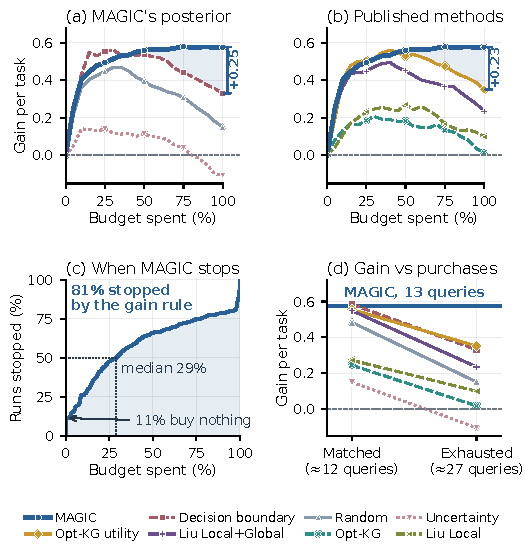
\includegraphics[width=\columnwidth]{budget_curves.pdf}
\caption{Acquisition rules versus the post-training budget spent (585 runs). (a) Rules sharing MAGIC's posterior and delivery rule; Uncertainty averages five uncertainty rules. (b) Adapted published methods; Opt-KG (vote delivery) and Kapoor VOI lie below the axis. (c) CDF of the budget share MAGIC has spent when it stops. (d) Gains at MAGIC's query count and at budget exhaustion; the line marks MAGIC.}
\label{fig:budget}
\end{figure}

\subsection{RQ3: Prior Sensitivity}
We test each of $\gamma$, $\alpha$, and $\beta$ at 0\%, 12.5\%, 25\%, 37.5\%, 50\%, 62.5\%, 75\%, 87.5\%, and 100\%, retaining the existing $\gamma=10\%$ result as well. Each sweep changes one parameter while holding the others at their defaults. Fig.~\ref{fig:parameters}a--c reports the gains and marks the highest observed mean in each grid with a star; Fig.~\ref{fig:parameters}d compares the nonnegative rates at these maxima with the default.

\begin{figure}[t]
\centering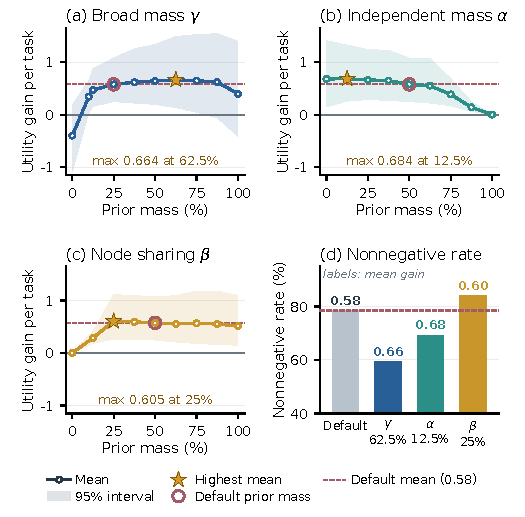
\includegraphics[width=\columnwidth]{prior_curves.pdf}
\caption{Prior sensitivity (585 runs). (a)--(c) Utility gain versus $\gamma$, $\alpha$, and $\beta$; stars: highest means; red circles: defaults; shading: 95\% intervals; dashed: default mean. (d) Nonnegative rate of the default and of each best setting; dashed: default rate.}
\label{fig:parameters}
\end{figure}

The largest mean in each one-factor sweep occurs at $\gamma=0.625$ (gain 0.6640), $\alpha=0.125$ (0.6838), and $\beta=0.25$ (0.6047). The first two settings concentrate gains on fewer combinations: their nonnegative rates are 59.49\% and 69.23\%, against 78.46\% at the default. At $\beta=0.25$ the rate rises to 84.10\%. The endpoints $\alpha=1$ and $\beta=0$ both make tasks independent and yield zero gain, as predicted by~\eqref{eq:prior-transfer}. By contrast, changing $\gamma$ also changes the no-query calibration. Supplementary Table~\ref{supp-tab:intervals} gives the paired differences.

\subsection{RQ4: Economic and Robustness Sensitivity}
\label{sec:rq4}
Table~\ref{tab:sensitivity} summarizes changes to the monetary budget, gold prices, task-value dispersion, and gold-label noise. Budget settings use $15\tilde c$ and $60\tilde c$. Price settings multiply all gold prices, including training prices, by 0.1, 0.25, 0.5, or 2 while keeping the original monetary budget fixed. Every configuration was checked for training-cost feasibility before execution.

\begin{table}[t]
\caption{MAGIC under economic and robustness changes (195 combinations). Gains are per task relative to each setting's no-query reference; CI: cluster bootstrap; new queries exclude prepaid training. Noisy-gold rows charge delivered corrupted labels the task's mean or maximum loss.}
\label{tab:sensitivity}\centering\smalltable\setlength{\tabcolsep}{2.5pt}
\begin{tabular}{lrrrr}
\toprule
Setting & Gain & 95\% CI & +/0/$-$ & New queries \\
\midrule
Default & 0.5767 & $[0.2501, 1.0763]$ & 135/18/42 & 13.19 \\
\midrule
\multicolumn{5}{l}{\emph{Total budget}} \\
$B=15\tilde c$ & 0.5579 & $[0.2380, 1.0607]$ & 136/18/41 & 8.83 \\
$B=60\tilde c$ & 0.5834 & $[0.2534, 1.0805]$ & 136/18/41 & 17.35 \\
\midrule
\multicolumn{5}{l}{\emph{Gold-price multiplier}} \\
$\times0.1$ & 3.1014 & $[1.9121, 4.9673]$ & 195/0/0 & 199.87 \\
$\times0.25$ & 2.0414 & $[1.1117, 3.6079]$ & 195/0/0 & 101.08 \\
$\times0.5$ & 1.1256 & $[0.5887, 2.0121]$ & 192/0/3 & 50.72 \\
$\times2$ & 0.2993 & $[0.0746, 0.5858]$ & 96/43/56 & 5.38 \\
\midrule
\multicolumn{5}{l}{\emph{Task-value dispersion}} \\
$\lambda=0$ & 1.0029 & $[0.1998, 2.3642]$ & 104/26/65 & 10.32 \\
$\lambda=0.5$ & 0.8799 & $[0.2199, 1.9348]$ & 127/12/56 & 13.81 \\
$\lambda=1.5$ & 0.2295 & $[0.0565, 0.4873]$ & 106/23/66 & 8.22 \\
\midrule
\multicolumn{5}{l}{\emph{Gold-label noise, mean loss}} \\
$\varepsilon=5\%$ & 0.5030 & $[0.1581, 1.0745]$ & 106/18/71 & 11.91 \\
$\varepsilon=10\%$ & 0.3660 & $[0.0361, 0.8994]$ & 83/18/94 & 11.74 \\
$\varepsilon=20\%$ & 0.2240 & $[-0.1412, 0.8428]$ & 53/18/124 & 10.87 \\
\midrule
\multicolumn{5}{l}{\emph{Gold-label noise, maximum loss}} \\
$\varepsilon=5\%$ & 0.4594 & $[0.1254, 1.0070]$ & 102/18/75 & 11.91 \\
$\varepsilon=10\%$ & 0.2844 & $[-0.0558, 0.7921]$ & 73/18/104 & 11.74 \\
$\varepsilon=20\%$ & 0.0767 & $[-0.3282, 0.6663]$ & 45/18/132 & 10.87 \\
\bottomrule
\end{tabular}
\end{table}

\paragraph{Budget}
Halving the budget retains 96.74\% of the default mean gain: 0.5579 versus 0.5767. Doubling the budget gives a gain of 0.5834 and ties MAGIC on 132 combinations. Both paired intervals include zero. The halved and doubled budgets use 58.00\% and 27.44\% of their amounts, with 9.60 and 18.12 total queries. Together with the default budget utilization of 42.26\%, these results indicate that the positive-gain stopping rule, not the budget, often determines the number of purchases.

\paragraph{Gold prices}
Halving gold prices makes about half of the prices lower than their rewards and raises the mean gain to 1.1256, with 192 positive and three negative combinations. Mean total queries increase from 13.96 to 51.49, and new expenditure rises from 0.1776 to 0.8321. Doubling prices gives a mean gain of 0.2993, with 96 positive, 43 tied, and 56 negative combinations. Gold prices thus act jointly on purchasing capacity, query selection, and posterior updates.

\paragraph{Cheaper gold labels}
At price multipliers of 0.25 and 0.1, a verified label can pay for itself directly. MAGIC gains 2.0414 and 3.1014, improves all 195 combinations in both settings, and makes 101.08 and 199.87 new queries. Random and cost-normalized uncertainty acquisition with MAGIC's posterior, run at MAGIC's query count or until budget exhaustion, trail MAGIC by 0.3270--0.5258, and all eight paired intervals exclude zero. New verification cost peaks at 0.9494 at multiplier 0.25; at 0.1, twice as many purchases cost 0.5635. The advantage therefore does not depend on the default regime with $c_i>r_i$.

\paragraph{Joint loss and price scaling}
Price changes alone leave wrong-label losses fixed. We therefore multiply every wrong-label loss by $\lambda_L\in\{0.25,0.5,1,2,4\}$ and every gold price, including training prices, by $m\in\{0.25,0.5,1,2\}$, keeping the monetary budget fixed (11,115 new runs). Because $\lambda_L$ moves the delivery threshold, each cell uses its own no-query reference, and gains are compared within, not across, loss scales. The mean gain is positive in all 20 cells (Fig.~\ref{fig:loss_price}), and 12 remain significant after Holm correction, including all ten with $m\le0.5$, where gains range from 0.2706 to 2.5157. Gains increase as gold labels become cheaper or errors more costly; for $m\le1$, they change by at most 0.0620 between $\lambda_L=2$ and 4. Doubling prices gives 0.0065--0.4750, with a median of zero and no significant cell, and at $\lambda_L=0.25$ the original prices give only 0.0402. Supplementary Section~\ref{supp-app:supporting} details the grid.

\begin{figure}[t]
\centering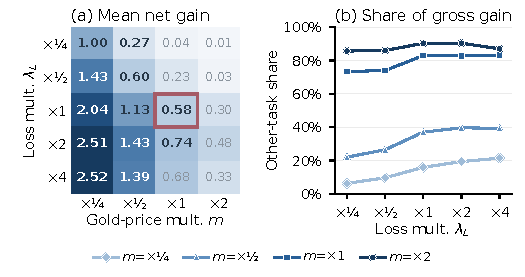
\includegraphics[width=\columnwidth]{loss_price.pdf}
\caption{Joint scaling of wrong-label losses $\lambda_L$ and gold prices $m$ at a fixed budget. (a) Mean net gain per task; bold: Holm-adjusted $p<0.05$; gray: not significant; red frame: main setting. (b) Share of gross gain from other tasks, one line per gold-price multiplier $m$.}
\label{fig:loss_price}
\end{figure}

\paragraph{Imperfect verification}
We corrupt each purchased label independently of query order, replacing it with a uniformly selected incorrect class with probability $\varepsilon$. When MAGIC treats the returned label as correct, gains under the mean wrong-label loss fall from 0.5767 at zero noise to 0.2240 at 20\% noise. Charging the maximum loss reduces the latter to 0.0767, with 132 of 195 combinations declining (Fig.~\ref{fig:noise}).

With the correct 20\% noise rate in its likelihood, MAGIC buys 6.64 labels per run, down from about 10.9, and acquires 1.29 corrupted labels versus 2.17. Its maximum-loss gain is 0.0976 (95\% CI $[0.0228,0.1823]$), while its mean-loss gain falls to 0.0996. Assuming half the true rate gives the largest means under both accounting rules, although the paired differences from the original model do not survive Holm correction. Supplementary Section~\ref{supp-app:supporting} specifies the observation channel and the experiments.

\begin{figure}[t]
\centering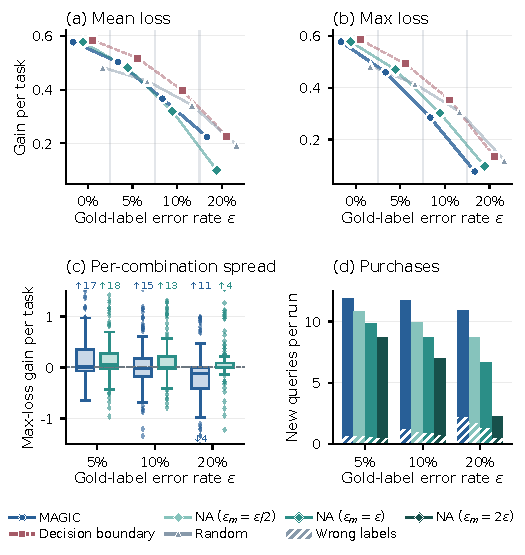
\includegraphics[width=\columnwidth]{noisy_gold.pdf}
\caption{Gold-label noise (585 runs). NA: noise-aware MAGIC with assumed error rate $\varepsilon_m$. (a)--(b) Gains when a delivered corrupted label is charged the task's mean or maximum loss. (c) Per-combination maximum-loss gains of MAGIC and NA ($\varepsilon_m=\varepsilon$). (d) New queries per run; hatching: corrupted labels.}
\label{fig:noise}
\end{figure}

\subsection{RQ5: Mechanism, Calibration, and Failures}
\label{sec:rq5}
\paragraph{Realized gain decomposition}
Using the common no-query delivery set, we separate purchased-task corrections, changes to the delivery of other tasks, and new verification cost. The identity is checked for every run. For full MAGIC,
\begin{equation}
 \underbrace{0.12870}_{\text{direct}}+
 \underbrace{0.62554}_{\text{other tasks}}-
 \underbrace{0.17756}_{\text{cost}}=
 \underbrace{0.57668}_{\text{net gain}}.
\end{equation}
Changes to other tasks contribute 82.94\% of the gross gain, which confirms the role of shared evidence in the default high-cost setting. Under the joint loss and price grid (Fig.~\ref{fig:loss_price}b), this share is 6.2\%--21.4\% at $m=0.25$ and 73.4\%--90.4\% at $m\ge1$: cheap labels are bought mainly for their direct return, whereas expensive labels pay off through transfer. On synthetic crowdsourcing pools, the share ranges from 8.9\% to 74.7\% with upstream quality and dependence strength (Supplementary Section~\ref{supp-app:supporting}). The Supplementary Material, Section~\ref{supp-app:accounting}, defines this decomposition and reports cumulative-gain trajectories.

\paragraph{Pool size and amortization}
To test whether transfer strengthens with pool size, we subsample the six largest pools (Senti, Web, ZenCrowd\_all, ZenCrowd\_in, ZenCrowd\_us, and product) to $n'\in\{100,250,500,1000,2000,4000\}$ tasks with $n'\le0.9n$, three replicates per size, and paid training tasks retained (3,276 runs). Upstream predictions and task economics are inherited from the full pool, the budget follows the main rule of 30 median subset prices, and each subset has its own no-query reference. Gains generally rise with $n'$ (Fig.~\ref{fig:pool_size}): Web increases from 0.2496 at $n'=100$ to 0.9111 at $n'=2000$, and product from 0.2725 to 0.4663 at $n'=4000$. On every pool, the ratio of other-task gain to new verification cost is higher on the full pool than at $n'=100$; on product it grows from 2.58 to 16.84. On ZenCrowd\_in and ZenCrowd\_all, the ratio stays below one up to $n'=1000$, and the gains at $n'=100$ are $-0.1156$ and $-0.0372$, with ZenCrowd\_in declining for all 13 baselines. On the full pools, the same two datasets gain 0.1787 and 0.1373. Small pools thus cannot amortize the verification cost, consistent with the negative gain on Bird ($n=108$).

\begin{figure}[t]
\centering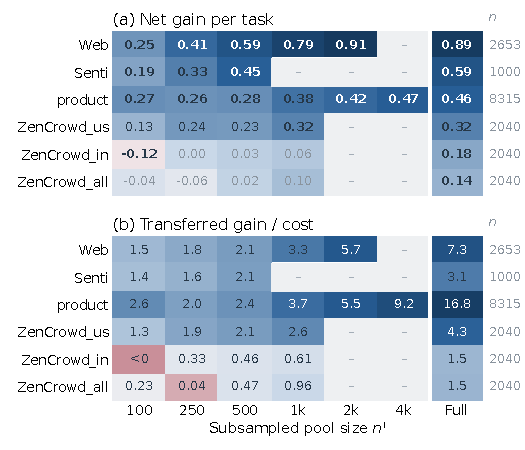
\includegraphics[width=\columnwidth]{pool_size.pdf}
\caption{Pool-size subsampling on the six largest pools. Full: complete pool, whose size $n$ is given at the right; ``--'': not subsampled ($n'>0.9n$). (a) Net gain per task; bold: 95\% bootstrap interval excludes zero. (b) Ratio of other-task gain to new verification cost.}
\label{fig:pool_size}
\end{figure}

\paragraph{Calibration on the same remaining tasks}
We compare baseline probabilities, MAGIC's prior probabilities, and its final posterior on the same final unqueried tasks in each run (Fig.~\ref{fig:calibration}). Mean multiclass Brier scores are 0.4438, 0.4104, and 0.3675; 10-bin ECE values are 0.1982, 0.1736, and 0.1138. Relative to the baseline probabilities, the final posterior reduces the Brier score by 17.19\% and ECE by 42.58\%, where reductions are computed from the unrounded mean scores. The evaluation set follows the adaptive query policy.

\begin{figure}[t]
\centering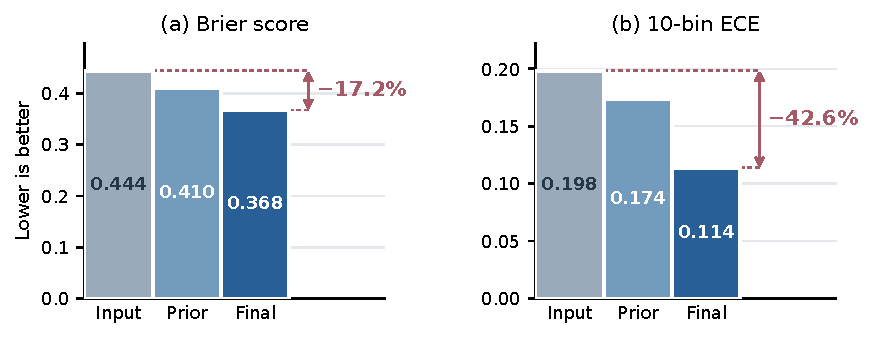
\includegraphics[width=\columnwidth]{calibration.pdf}
\caption{Calibration on the final unqueried tasks (lower is better). Arrows: change from baseline probabilities to MAGIC's posterior.}
\label{fig:calibration}
\end{figure}

\paragraph{Limited scope for profitable revision}
For each combination, we measure the decision headroom before querying as the loss from incorrectly delivered labels plus the reward of correctly predicted but rejected labels, per task. This quantity separates opportunities to change delivery from overall prediction accuracy. The lowest-headroom quartile gains 0.1212 and contains 17 negative combinations out of 49; the highest quartile gains 1.8134 and contains three out of 48. The Spearman association of headroom with gain is 0.482, compared with $-0.066$ for accuracy (Fig.~\ref{fig:mechanism}b). Grouping by accuracy shows no increasing pattern: the lowest-accuracy quartile gains 1.2501 and the highest 0.4949 (Fig.~\ref{fig:mechanism}c). Accurate predictions can still benefit when their confidence causes unnecessary rejection; headroom and the cost of learning how to use it are more informative diagnostics than accuracy.

\begin{figure}[t]
\centering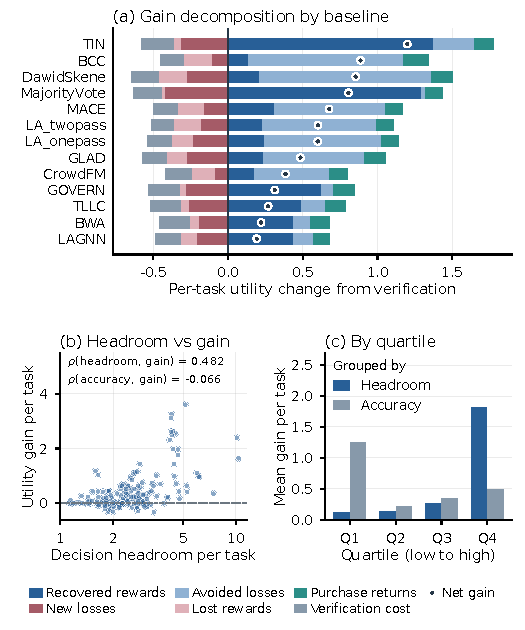
\includegraphics[width=\columnwidth]{mechanism.pdf}
\caption{Sources of MAGIC's gain (195 combinations). (a) Per-task gain decomposition by baseline; dots: net gain. (b) Utility gain versus decision headroom (log scale); six combinations with gains above 4 are omitted. (c) Mean gain by quartile of headroom and of baseline accuracy.}
\label{fig:mechanism}
\end{figure}

\paragraph{Costly delivery revisions}
Two failure cases show how transfer can go wrong in either direction. CF/CrowdFM illustrates costly delivery revisions by the shared posterior despite 88.33\% baseline accuracy and 0.5480 of incorrect-delivery loss before querying. On average, about one newly delivered incorrect label incurs a loss of 0.3213 per pool task, exceeding the 0.2176 benefit from favorable changes to other deliveries. Bird/BWA exhibits overly conservative transfer: the rejected set has posterior expected utility of $-0.0451$ per pool task but realized utility of 0.2311, which rejection forgoes. Lost correct-label rewards amount to 0.4087, alongside verification costs of 0.2825. Supplementary Table~\ref{supp-tab:failures} reports these harmful revisions for the five lowest-gain combinations.

\paragraph{Task values and decision thresholds}
Using the coefficient of variation of reward plus mean wrong-label penalty, the lowest-dispersion quartile has five negative combinations out of 49, compared with 15 out of 48 in the highest quartile. The rank correlation with gain is $-0.264$. Even equal-value tasks can benefit from verification when their correctness probabilities lie on different sides of the delivery threshold. A controlled experiment tests the role of dispersion by rescaling rewards and wrong-label losses within each pool in log space by a factor $\lambda$ while preserving their arithmetic means. Gains decrease from 1.0029 at $\lambda=0$ (equal values) to 0.8799, 0.5767, and 0.2295 at $\lambda=0.5$, 1 (original), and 1.5 (Table~\ref{tab:sensitivity}); each remains positive with cluster $p<0.008$. Each gain uses the no-query reference at the same dispersion. The controlled result agrees with the observed negative association in mean gain. At $\lambda=0$, however, the gain concentrates on fewer combinations: 65 decline, compared with 42 at $\lambda=1$.

% ===== DISCUSSION =====
\section{Discussion}
\label{sec:discussion}
\paragraph{Different baselines leave different decisions to improve}
In Fig.~\ref{fig:mechanism}a, recovered rewards are rewards of correct labels that the reference rejected but MAGIC delivers, and avoided losses are losses of incorrect labels that the reference delivered but MAGIC rejects. TIN and MajorityVote obtain large gains by recovering correct answers that the reference rejects. Their mean baseline confidences are 0.5922 and 0.6096, and the reference delivers 30.04\% and 33.67\% of untrained tasks. Subsequent delivery of previously rejected correct labels contributes 1.3768 and 1.2970, respectively, before subtracting harmful changes and verification cost. TIN's 167.43\% relative gain also reflects its reference utility of 0.7165. BWA starts from 1.9875 and gains 0.2223, or 11.19\%; its smaller gain combines a stronger reference with less beneficial transfer and a verification cost of 0.1966.

BCC and Dawid--Skene show the opposite mechanism. Their mean confidences are 0.9703 and 0.9646, while their mean accuracies are 73.73\% and 72.78\%. The reference therefore delivers many predictions exposed to substantial error penalties, and rejecting previously delivered incorrect labels after verification recovers 1.0364 and 1.1478. Thus, the large gains of TIN/MajorityVote and BCC/Dawid--Skene arise from opposite delivery adjustments, recovering overly cautious rejections and suppressing costly errors, visible as the dark and light blue segments in Fig.~\ref{fig:mechanism}a. The probability interface, together with task economics, determines which adjustment is valuable.

LAGNN and TLLC gain 0.1931 and 0.2697. Their favorable changes to unpurchased deliveries contribute 0.5713 and 0.6538, but harmful changes consume 0.3134 and 0.3138, leaving 0.2579 and 0.3400 of other-task gain. Their verification costs of 0.1719 and 0.2052 further reduce the net benefit. These outcomes explain why a more elaborate prediction model can still have a modest verification gain: its errors, confidence, and transferable corrections need to align with the economic decision.

\paragraph{Dataset gains reflect distinct opportunities for sharing}
Valence7's large gain is driven by avoided error penalties. Baseline accuracy averages 20.69\%, and the reference incurs 4.7273 of incorrect-delivery loss. Subsequent rejection of incorrect predictions saves 4.0474; after other changes, other-task gain is 3.5636. Web benefits primarily from recovering correct answers: the reference forgoes 2.8460 of correct-label rewards, and later delivery recovers 1.3348. These two datasets illustrate why low accuracy and excessive caution can both create substantial economic improvement.

Product has 90.42\% mean accuracy yet gains 0.4569. Its other-task gain is 0.4662 and its verification cost is 0.0277, consistent with sharing the benefit of a few observations over a large pool. Subsampling confirms this mechanism (Fig.~\ref{fig:pool_size}). Bird has only 108 tasks: its gross gain of 0.1335 falls short of the 0.1488 verification cost. Subsampled ZenCrowd pools of 100--250 tasks show the same shortfall. UC makes no additional purchases; only 7.85\% of tasks have prior expected utility within 10\% of their reward-plus-penalty scale of the decision boundary. Together with its zero-query traces, this is consistent with limited model-estimated opportunity to change delivery profitably, even though its mean prediction accuracy is only 63.31\%.

\paragraph{Predicted and realized return}
The left panel of Fig.~\ref{fig:synthetic} tests the cumulative identity~\eqref{eq:cumulative} on labels sampled from the MAGIC prior. Across 100 pools per class count, the mean realized gain minus the sum of predicted gains, both per task, is $-0.0436$ for two classes and $+0.0464$ for three. Both bootstrap intervals include zero, although 43--44\% of individual pools lose utility. In a separate worker simulation, calibration varies by latent group. At matched query counts, MAGIC exceeds the decision-boundary heuristic by 0.0721--0.3772 per task across all 16 settings and exceeds random selection in every setting. Supplementary Section~\ref{supp-app:supporting} specifies the two generating processes.

\begin{figure*}[t]
\centering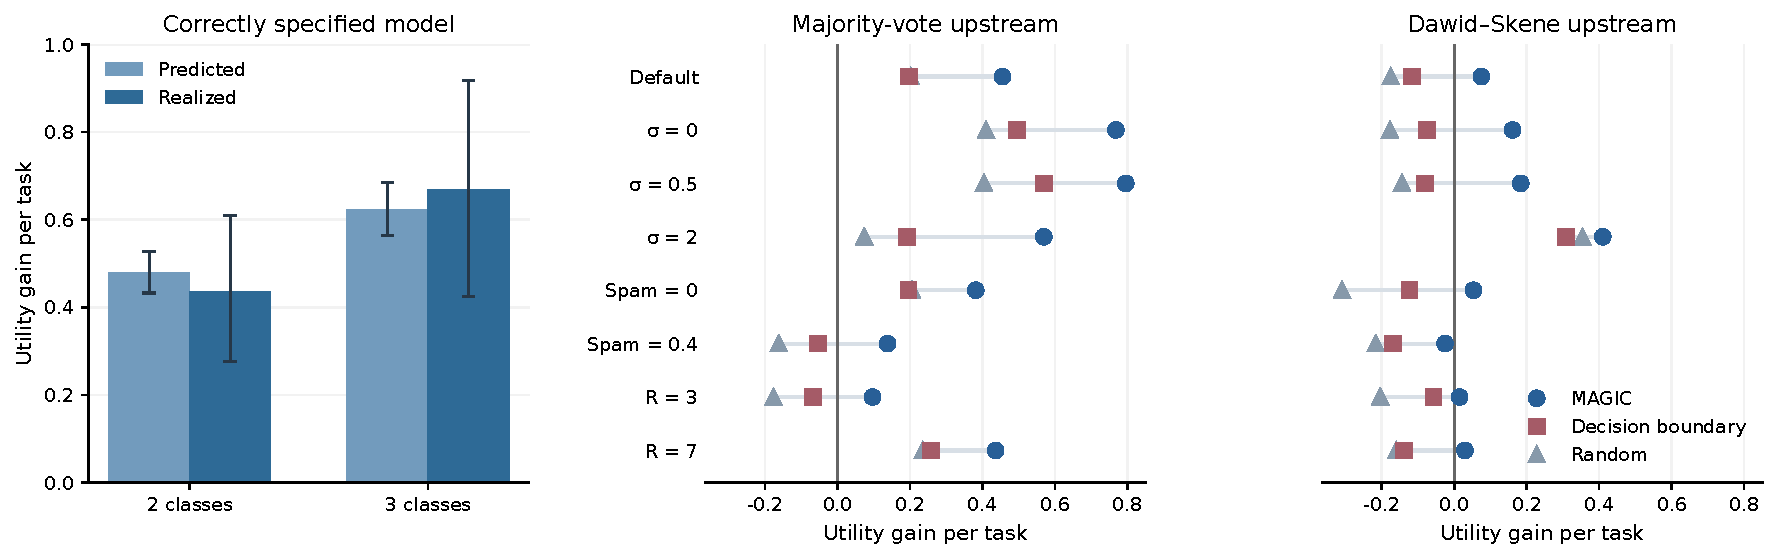
\includegraphics[width=\textwidth]{synthetic.pdf}
\caption{Synthetic validation. Left: predicted (sum of one-step gains) and realized gains on correctly specified pools, with 95\% bootstrap intervals over pools. Middle and right: gains of MAGIC, the decision-boundary heuristic, and random selection at MAGIC's query count under majority-vote and Dawid--Skene upstreams; each row varies one factor from the default.}
\label{fig:synthetic}
\end{figure*}

\paragraph{Verification beyond one step}
A first observation can reveal a profitable follow-up purchase. On the six pools small enough for the two-step comparison, a restricted two-step search increases mean gain by 0.0685 (95\% CI $[-0.0320,0.2126]$) and makes 4.40 purchases on average versus 3.76. It improves 20 of 78 combinations and trails on 52. This variation makes the size and location of a downstream delivery change important when deciding how far to plan.

\section{Conclusion}
\label{sec:conclusion}
MAGIC prices a gold label by the return on its own task and the delivery decisions it can change elsewhere. Its context model learns which tasks share calibration, and its one-step score measures how far an observation can move those tasks across the delivery threshold. Across 15 datasets the average gain is 0.5767 per task. Expensive gold earns most of its return through changes on other tasks, while cheaper gold shifts the balance toward direct corrections.

\bibliographystyle{IEEEtran}
\bibliography{references}
\end{document}
